\documentclass[a4paper,oneside]{article}
\usepackage[french]{babel}
\usepackage[utf8]{inputenc}
\usepackage{hyperref} % références dans pdf
\usepackage[tt]{titlepic}
\usepackage{graphicx} % pour images
\usepackage{rotating} % pour
\usepackage{lmodern}
\usepackage{amsmath}
\usepackage{amssymb}
\usepackage{mathrsfs}
\usepackage{sistyle}
\usepackage{chngpage}
\usepackage{epstopdf}
\usepackage{gnuplottex}% pour faire du gnuplot directement dans le latex, finalement pas utilisé, résultats pas assez beaux 
\usepackage[nottoc, notlof, notlot]{tocbibind} % pour que bibliographie soit comprise comme un chapitre ou section
\usepackage{appendix} % pour les annexes
%\pagestyle{headings} % pour en têtes

\makeatletter % pour /bigcenter qui permet de s'affranchir des marges pour les images
 
\newskip\@bigflushglue \@bigflushglue = -100pt plus 1fil
 
\def\bigcenter{\trivlist \bigcentering\item\relax}
\def\bigcentering{\let\\\@centercr\rightskip\@bigflushglue%
\leftskip\@bigflushglue
\parindent\z@\parfillskip\z@skip}
\def\endbigcenter{\endtrivlist}
 
\makeatother

\begin{document}

%************************************************************************
%									TITRE
%************************************************************************


\begin{titlepage} % Suppresses headers and footers on the title page

	\centering % Centre everything on the title page

	\scshape % Use small caps for all text on the title page

	\vspace*{\baselineskip} % White space at the top of the page


	\rule{\textwidth}{1.6pt}\vspace*{-\baselineskip}\vspace*{2pt}
	 % Thick horizontal rule
	\rule{\textwidth}{0.4pt} % Thin horizontal rule

	\vspace{0.75\baselineskip} % Whitespace above the title

	{\LARGE RAPPORT DE VALIDATION :\\ PROFILS NACA\\} % Title

	\vspace{0.75\baselineskip} % Whitespace below the title
	\rule{\textwidth}{0.4pt}\vspace*{-\baselineskip}\vspace*{3.2pt}
	 % Thin horizontal rule
	\rule{\textwidth}{1.6pt} % Thick horizontal rule
	\vspace{2\baselineskip} % Whitespace after the title block

	%------------------------------------------------
	%	Subtitle
	%------------------------------------------------

	% Subtitle or further description
	Calculs Scientifiques \& Programmation

	\vspace*{3\baselineskip} % Whitespace under the subtitle

	%------------------------------------------------
	%	Editor(s)
	%------------------------------------------------


	\vspace{0.5\baselineskip} % Whitespace before the editors

	{\scshape\Large Quentin Bergé } % Editor list

	\vspace{0.5\baselineskip} % Whitespace below the editor list

	\textit{ENSEEIHT} % Editor affiliation

	\vfill % Whitespace between editor names and publisher logo

	%------------------------------------------------
	%	Publisher
	%------------------------------------------------

	
\includegraphics[scale=0.3]{logoN7.png} % changer logo

	\vspace{0.3\baselineskip} % Whitespace under the publisher logo

Novembre 2018 % Publication year

	

\end{titlepage}
\newpage
%*******************************************************
% DEBUT RAPPORT
%********************************************************


\section{Introduction}
Il est question ici d'utiliser un programme pour effectuer le calcul des profils d'ailes NACA dont les paramètres sont définis dans l'énoncé de TP ainsi qu'avec les ressources du site airfoiltools et l'article Profils NACA tiré du site Wikipedia.

\section{Contenu}

Le programme est placé dans le dossier Fortran qui comprend :

\begin{itemize}
	\item un fichier \verb?module_tp4.f90? % pour ne pas tenir compte de la mise en forme du texte très utile !!!
	\item un fichier de subroutines \verb?subroutines.f90?
	\item le programme \verb?tp4.f90?
	\item le fichier \verb?Makefile? permettant la compilation\\
	\end{itemize}

Le dossier RUN comprend :
\begin{itemize}
	\item les fichier de sorties de forme \verb?tp4_NACA_XXXXX_npt_XXXX_.out?
	\item le fichier d'entrée \verb?profil.in?
	\item le programme compilé \verb?tp4.bin?\\
\end{itemize}

Dans le dossier Validation sont compris :
\begin{itemize}
	\item les fichiers de résultats issus du site \textit{airfoiltools.com} qui seront utilisés pour la comparaison pour les différents profils nommés de la forme \verb?AirfoilXXXXX.out?
	\item les résultats du programme pour les différents profils
	\item les graphiques des différents profils\\
\end{itemize}

Le dossier $\LaTeX$ comprend les ressources pour le rapport ainsi que le rapport en lui-même.

\section{Validation}
\`A l'aide des valeurs de référence fourni par \textit{airfoiltools.com} j'ai pu confronter les données de sorties de mon programme pour 4 différents types de profils. Les résultats de notre programme ont été exprimés avec 150 points.

\subsection{NACA0012}

\begin{figure}[h!]
\bigcenter
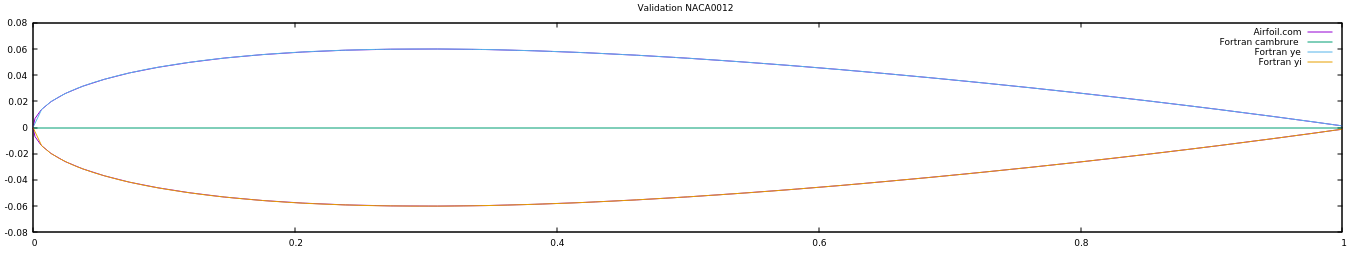
\includegraphics[scale=0.4]{Validation0012.png}
\caption{Comparaison des résultats pour NACA0012}
\end{figure}

En orange et en bleu sont représentés respectivement l'extrados et l'intrados, en vert est représentée la $cambrure$ et en violet les résultats de référence pour le profil considéré.

Les résultats de références et les résultats issus du programme semblent parfaitement correspondre sur la totalité du profil. 

\begin{figure}[h!]
\centering
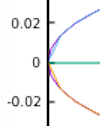
\includegraphics[scale=0.4]{decalage0.png}
\caption{Décalage en $x=0$ }
\end{figure}

Néanmoins, on peut observer un très léger décalage entre les résultats de références et les résultats issus du programme sur le tout début du profil. Ce décalage reste inexpliqué pour le moment.
\begin{table}[h!]
\begin{center}
\begin{tabular}{|c|c|c|c|c|}
	\hline
   $x$ & $x_e$ & $x_i$ & $y_e$ & $y_i$\\
   \hline
   0,1E+01 & 0,1E+01 & 0,1E+01 & -0,126E-02 & 0,126E-02 \\
   \hline
   
\end{tabular}
\caption{Dernières valeurs des résultats du programme de NACA0012}
\end{center}
\end{table}

De plus, en analysant les résultats de la fin du profil, on peut observer que les valeurs des ordonnées de l'extrados et de l'intrados du fichier de sortie ne rejoignent pas parfaitement 0. Il s'agit en effet d'une erreur sur le bord de fuite qui est aussi présent sur le fichier des résultats de référence d'airfoiltools, c'est pour cela que nous ne voyons pas de différences notables sur les images.


Ces deux erreurs sont présentes pour tous nos résultats suivants.


\subsection{NACA4412}

\begin{figure}[h!]
\bigcenter
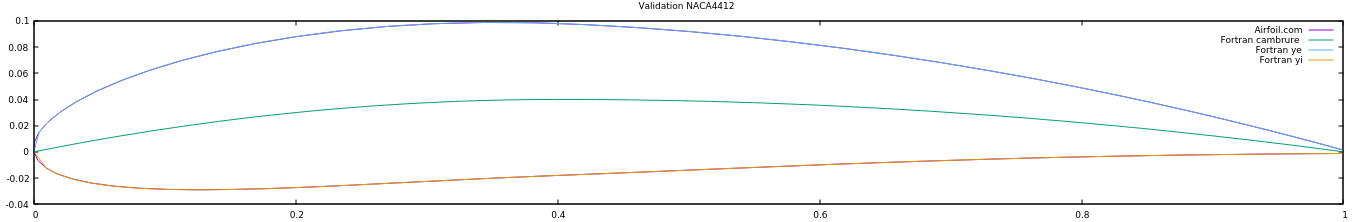
\includegraphics[scale=0.4]{Validation4412.png}
\caption{Comparaison des résultats pour NACA4412}
\end{figure}

En orange et en bleu sont représentés respectivement l'extrados et l'intrados, en vert est représentée la $cambrure$ et en violet les résultats de référence pour le profil considéré.

\`A l'instar des résultats précédents, on observe une correspondance parfaite sur la quasi-totalité du profil excepté pour le tout début où l'on peut distinguer un très léger décalage.
\newpage
\subsection{NACA23012}

\begin{figure}[h!]
\bigcenter
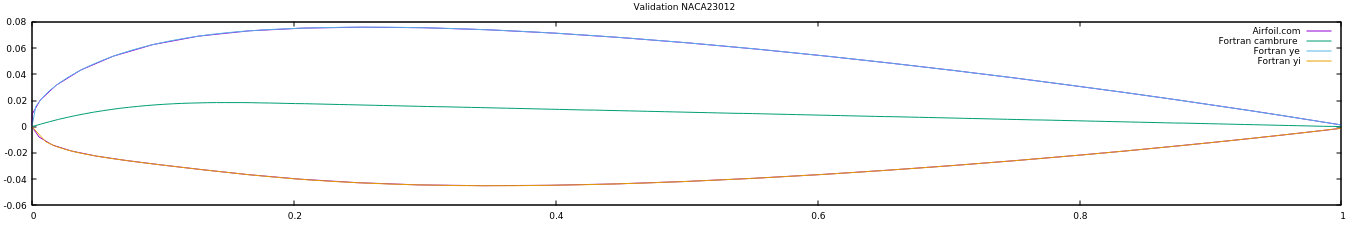
\includegraphics[scale=0.4]{Validation23012}
\caption{Comparaison des résultats pour NACA23012}
\end{figure}

En orange et en bleu sont représentés respectivement l'extrados et l'intrados, en vert est représentée la $cambrure$ et en violet les résultats de référence pour le profil considéré.

Nous pouvons observer les mêmes phénomènes que pour les résultats précédents.

\subsection{NACA23112}


\begin{figure}[h!]
\bigcenter
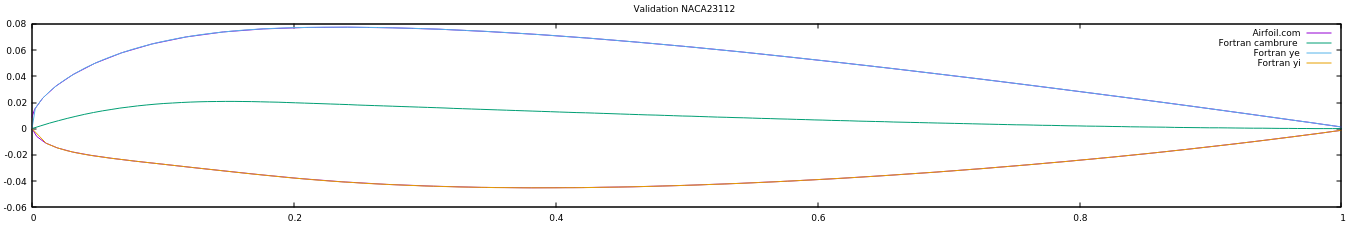
\includegraphics[scale=0.4]{Validation23112.png}
\caption{Comparaison des résultats pour NACA23112}
\end{figure}



%\begin{figure}[htbp]
%\centering
%\begin{gnuplot}[terminal=latex]
%set size 1,1; set title "Validation NACA23112";  plot "Airfoil_23112.out" using 1:2 title "Airfoil.com" with lines lt rgb "violet", "tp4_NACA_23112_npt_00150.out" using 2:7 title "Fortran cambrure" with lines, "tp4_NACA_23112_npt_00150.out" using 4:6 title "Fortran ye" with lines, "tp4_NACA_23112_npt_00150.out" using 3:5 title "Fortran yi" with lines
  
%  
%\end{gnuplot}
%\end{figure}



En orange et en bleu sont représentés respectivement l'extrados et l'intrados, en vert est représentée la $cambrure$ et en violet les résultats de référence pour le profil considéré.

Ici aussi, Nous pouvons observer les mêmes phénomènes que pour les résultats précédents.
\section{Conclusion}

En somme, le programme produit de très bons résultats sur la totalité du profil et ceci dans les 4 cas étudiés c'est-à-dire pour NACA 4 et 5 chiffres. Compte tenu de ces résultats vis-à-vis des résultats de référence, nous pouvons valider notre programme. 


Le léger décalage observé en début de profil et l'erreur du bord de fuite à la fin du profil restent pour l'heure inexpliqués et sont communs à plusieurs étudiants de la classe. Il serait intéressant de trouver l'origine de ces erreurs, l'erreur de bord de fuite pourrait être minimisée en augmentant la longueur de la corde.


 \end{document}
  